% pdflatex -shell-escape nystsin 

\documentclass[t]{beamer}
\usepackage[utf8]{inputenc}

\usepackage{../templates/beamerthemeCCM}
\usepackage{epstopdf}  % handle EPS
\usepackage{bm}
\usepackage{multirow}

\usepackage{tikz}
\usetikzlibrary{shapes.geometric, arrows}

% alex macros
\input{../templates/rgb}
\newcommand{\ft}[1]{\frametitle{#1}}
\newcommand{\bi}{\begin{itemize}}
\newcommand{\ei}{\end{itemize}}
\newcommand{\ben}{\begin{enumerate}}
\newcommand{\een}{\end{enumerate}}
\newcommand{\be}{\begin{equation}}
\newcommand{\ee}{\end{equation}}
\newcommand{\ba}{\begin{align}}
\newcommand{\ea}{\end{align}}
\newcommand{\bc}{\begin{center}}
\newcommand{\ec}{\end{center}}
\newcommand{\mbf}[1]{{\bm #1}}           % requires bm package
\newtheorem{thm}{Theorem}
\newcommand{\ig}[2]{\includegraphics[#1]{#2}}
\newcommand{\tbox}[1]{{\mbox{\tiny #1}}}
\newcommand{\who}[1]{{\scriptsize \textcolor{darkgreen}{(#1)}}}  % cite
\newcommand{\com}[1]{{\scriptsize \textcolor{purple}{#1}}}      % comment
\newcommand{\co}[1]{{\scriptsize \tt #1}}          % code
\newcommand{\vg}{\vspace{2ex}}
\newcommand{\sg}{\vspace{1ex}}
\newcommand{\hg}{\vspace{0.5ex}}
\newcommand{\dr}[1]{{\color{darkred}#1}}    % for bullets
\newcommand{\rb}{\ensuremath{\textcolor{darkred}{\bullet\;}}\ }
\newcommand{\gb}{\ensuremath{\textcolor{teal}{\bullet\;}}\ }
\newcommand{\bmp}[1]{\begin{minipage}{#1}}
\newcommand{\bmpt}[1]{\begin{minipage}[t]{#1}}
\newcommand{\emp}{\end{minipage}}
\newcommand{\pig}[2]{\bmp{#1}\includegraphics[width=#1]{#2}\emp} % mp-fig, nogap
\newcommand{\pigm}[3]{\bmp{#1}\href{#3}{\includegraphics[width=#1]{#2}}\emp} % w/ movie
\newcommand{\ora}[1]{{\color{orange} #1}}
\newcommand{\gre}[1]{{\color{green} #1}}
\newcommand{\yel}[1]{{\color{yellow} #1}}
\newcommand{\sr}[1]{{\scriptsize #1}}
\newcommand{\eps}{\epsilon}
\newcommand{\qqquad}{\qquad\qquad}
\newcommand{\qqqquad}{\qqquad\qqquad}
\newcommand{\R}{\mathbb{R}}
\newcommand{\Z}{\mathbb{Z}}
\newcommand{\N}{\mathbb{N}}
\newcommand{\emach}{\epsilon_\tbox{mach}}
\DeclareMathOperator{\im}{Im}
\DeclareMathOperator{\re}{Re}
\newcommand{\bigO}{{\cal O}}
\newcommand{\pO}{{\partial\Omega}}
\newcommand{\xx}{\mbf{x}}
\newcommand{\yy}{\mbf{y}}
\newcommand{\uu}{\mbf{u}}
\newcommand{\nn}{\mbf{n}}
\newcommand{\Srep}{{\cal S}}
\newcommand{\Drep}{{\cal D}}



\title{Overview of Nystr\"om high-order quadratures for boundary integral equations}
\date{Computational Tools 2024 BIE workshop. Day 1, 6/6/24}
\author{\textbf{Hai Zhu}\inst{1}}
\institute{\inst{1} Center for Computational Mathematics, Flatiron Institute, Simons Foundation}

\begin{document}

\begin{frame}
	\titlepage
\end{frame}


\begin{frame}\ft{Overview}

%%%
\bmp{3.2in}
Goal: evaluate layer potential 

\quad $u(\xx) = (K\sigma)(\xx) := \int_\Gamma k(\xx,\yy) \sigma(\yy) dS_\yy,
        \quad \xx \in\Omega$
\sg        

\rb
Two routes to discretizing $\Gamma$ and $\sigma$: 

\quad Global: efficient for simple, smooth geometries 

\qquad \com{trapezoidal rule, spherical harmonics}

\quad Local: adaptivity for complex geometries

\qquad \com{G-L panels, triangular/quadrilateral elements}

\rb
Two routes to discretizing the operator: 

\quad Galerkin: project integral operator onto a basis

\qquad \com{more mature convergence theory, industrial codes }

\quad Nystr\"om: approx. integral operator at quadr. points

\qquad \com{faster set-up, basically same accuracy at same order }

\sg

\rb Computational Tools: 

    \qquad chunkie (2D), fmm3dbie (3D), et al.
\emp

\hfill
\bmp{1.2in}
\vspace{-55ex}
\ig{width=1.1in}{fig_intro2d}

\ig{width=1.1in}{fig_intro3d}

\qquad \ig{width=0.7in}{peaked_kernel2d}

\quad \ig{width=1in}{peaked_kernel3d.pdf}

\quad \ig{width=1in}{geomellipsoid_terr.png}

\sg
\emp

\end{frame}

\begin{frame}\ft{Overview: local discretization and Nystr\"om}

\bmp{3.4in}
Goal: evaluate layer potential due to $\Gamma=\cup \gamma_m$

\quad $u(\xx)  = (K\sigma)(\xx) = \sum_m \int_{\gamma_m} k(\xx,\yy) \sigma(\yy) dS_\yy$

\quad \com{ in particular, compute $u(\xx)$ for $\xx \in \Gamma$ to get linear system for $\sigma$ }

\rb A sampling of integration ideas: 

    \qquad adaptive integration 

    \qquad generalized Gaussian quadr. 
    
    \qquad integration by parts 

\rb Discretizing operator $K$ : 

    \qquad on smooth curves is a solved problem

    \qquad on curves with corners is also no trouble

    \qquad on smooth surfaces \com{ currently is $10^3-10^4$ targs/sec/core }

    \qquad surfaces with singularities \com{ 3D corners, cones, and edges}

    \qquad related: high aspect ratio / skew panels
    
\sg

\begin{tikzpicture}[scale=0.5]
    \tikzstyle{box} = [rectangle, rounded corners, minimum width=3cm, minimum height=0.5cm,text centered, draw=black, fill=green!30]
    \scriptsize
    \node (center) [box] at (5,-1.4) {GGQ \& adaptive integration};
    \draw[->, thick] (0,-2) -- (10,-2) node[anchor=north] {};
    \node[anchor=north] at (1,-2) {regularization + asymptotics};
    \node[anchor=north] at (8,-2) {product integration};
    \node[anchor=west] at (10,-1) {chunkie};
    \node[anchor=west] at (10,-1.5) {fmm3dbie};
    \node[anchor=west] at (11,-2) {order};
\end{tikzpicture}

\emp

\hfill
\bmp{1.25in}
\vspace{-50ex}

\ig{width=1.4in}{2d_config}

\ig{width=1.4in}{3d_config}

\quad\small{1D integral}

\sg

\quad \com{weak: $\int_{\Gamma} \log|x-y|\, dy$} 

\quad \com{strong: $\int_{\Gamma} \frac{1}{|x-y|}\, dy$} 

\quad \com{hyper: $\int_{\Gamma} \frac{1}{|x-y|^2}\, dy$} 

\quad \com{super: $\int_{\Gamma} \frac{1}{|x-y|^3}\, dy$} 

\sg
\quad\small{2D integral}

\sg

\quad \com{weak: $\int_{\Gamma} \frac{1}{|x-y|}\, dy$} 

\quad \com{strong: $\int_{\Gamma} \frac{1}{|x-y|^2}\, dy$} 

\quad \com{hyper: $\int_{\Gamma} \frac{1}{|x-y|^3}\, dy$} 

\emp


\end{frame}

\begin{frame}\ft{Discretization of $\Gamma$ and $\sigma$}

\bmp{3.5in}
\rb 
(G) global: efficient for simple, smooth geometries 

    \ig{width=2.7in}{mesh_g}

\com{peri. trap. rule \qquad sph. harms. \qquad overlapping patches}

\hspace{0.8in} \who{Veerapaneni et al.} \quad \who{Ying et al.}

\rb 
(L) local: adaptivity for complex geometries


    \ig{width=2.7in}{mesh_l}
\emp

\com{G-L panels \hspace{0.4in} G-L quads \hspace{0.4in} 4th-ord tri's}

\hspace{0.8in} \who{Barnett et al.} \quad \who{Greengard et al.} \quad \com{industrial geoms.}

\hfill
\bmp{1.8in}
\vspace{-30ex}
\quad\ig{width=1.8in}{plane-dir-final}
\emp


\end{frame}

\begin{noframe}\ft{Quadrature literature}

{\scriptsize Auxiliary nodes/patches:} \who{Barnett-Greengard-Hagstrom '20, Greengard-O'Neil-Rachh-Vico '21}

{\scriptsize GGQ:} \who{Ma-Rokhlin-Wandzura '96; Yarvin-Rokhlin '98; Bremer '12; Bremer-Gimbutas-Rokhlin '10, Bremer-Gimbutas '12, ...}
        
{\scriptsize QBX and hedgehog:} \who{Kl\"ockner-Barnett-Greengard-O'Neil '13; Morse-Rahimian-Zorin '21; Af Klinteberg-Tornberg '16; Siegel-Tornberg '18; Wala-Kl\"ockner '18, ...}
  
{\scriptsize Change of variable/singularity cancelation:} \who{Ying-Biros-Zorin '06; Malhotra-Cerfon-Imbert-G\'erard-O'Neil '19; Erichsen-Sauter '98; Gimbutas-Veerapaneni '13, ...}

{\scriptsize Kernel regularization:} \who{Beale '01; Tlupova-Beale '19; P\'erez-Arancibia-Faria-Turc '18; Dong-Lai-Li '20; Bao-Xu-Yin '17 ...}

{\scriptsize Corner/Open surface:} \who{Helsing-Ojala '08; Helsing '11; Helsing-Jiang '18; Helsing-Jiang '22; Rachh-Serkh '17; Hoskins-Rachh '19; Bremer-Rokhlin-Sammis '10; Bremer-Rokhlin-Sammis '10; Serkh-Rokhlin '16; Gopal-Trefethen 19; Kress '90 ...}

{\scriptsize Kernel Split:} \who{Helsing-Karlsson '14; Helsing-Holst '15; Fryklund-Af Klinteberg-Tornberg '19 ...} 
        
{\scriptsize And many more}: \who{Kress '91; Alpert '95; Kapur-Rokhlin '97; Duan-Rokhlin '08; Kolm-Rokhlin '01; Wu-Martinsson '22; Xiao-Gimbutas '10; Bremer-Gimbutas '12; Barnett-Wu-Veerapaneni '15; Stein-Barnett '22; Af Klinteberg-Barnett '21; Af Klinteberg '23; Bao-Hua-Lai-Zhang '23; Malhotra-Barnett '23 ...}

\end{noframe}

\begin{frame}\ft{Quadrature tasks and categories}

\bmp{4.5in}
    \rb
    task A) fill $A^{\text{far}}$: \com{$|\xx_i-\xx_j|>d$, use smooth quadr, $A_{ij} = k(\xx_i,\xx_j) w_{j}$}

    \rb
    task B) fill $A^{\text{near}}$: \com{$|\xx_i-\xx_j|<d$, need near-singular quadr, $A_{ij} = k(\xx_i,\xx_j) w_{ij}$}

    \rb
    task C) fill $A^{\text{self}}$: \com{$\xx_i=\xx_j$, need singular quadr, $A_{ii} = k(\xx_i,\xx_i) w_{ii}$} 
\emp

\sg

\bmp{1.8in}
    \ig{width=1.8in}{taskfig1}
    \qquad\who{Martinsson '14 CBMS}
\emp
\hfill
\bmp{2.7in}
    \ig{width=2.7in}{taskfig2}
\emp

\sg
Quadrature wish list:
\sg

\bmp{2.5in}
    \rb
    dimension independent 2D and 3D

    \rb
    kernel independent

    \rb
    high order accurate to industrial mesh

    \rb
    setup speed

    \qquad \com{on-the-fly for moving geometry}
\emp
\hfill
\bmp{2in}
    \rb
    robust to target location

    \rb
    robust to patch deformation

    \rb
    parallel implementation

    \rb
    easy to use for non-expert 
    
    \qquad \com{soln. anywhere}
\emp

\end{frame}

\begin{frame}\ft{Quadrature task A) fill $A^{\text{far}}$}
$A_{ij} = k(\xx_i,\xx_j) w_j$, \com{$w_j$ independent of $\xx_i$} 

\sg 

$u(\xx) = \int_0^{2\pi} k(\xx,\yy(t))\sigma(t) |\yy'(t)|\, dt $

\sg 

parametric $\xx(t):$  \com{$(0,2\pi)\rightarrow \Gamma$}

global: \com{axisymmetric geoms.} 

\bmp{2.5in}
    \ig{width=0.8in}{taskA1}
    \ig{width=0.8in}{taskA2}
    \ig{width=0.8in}{taskA3}
\emp
\hfill
\bmp{2.2in}
\vspace{-35ex}

\hspace{-2ex} peri. trap. rule for peri. func.

\sg

\com{$t_j = 2\pi j/N, \sigma_j=\sigma(t_j),$ for $ j=1,\cdots,N $}

\sg

\com{$w_j = |\xx'(t_j)|\cdot 2\pi/N$, arc length}

\sg
\com{$A_{ij} = k(\xx_i,\xx_j)w_j$, if $|\xx_i-\xx_j|>d$}

\emp

\sg

\pause

local: 

\bmp{2.5in}
    \ig{width=0.8in}{taskA4}
    \ig{width=0.8in}{taskA5}
    \ig{width=0.8in}{taskA6}
    
    \hspace{22ex} \who{Vioreanu-Rokhlin} 
\emp

\hfill
\bmp{2.2in}
\vspace{-32ex}

$p-$point G-L nodes and weights

\sg

$\Gamma=\cup \gamma_m$, each $\gamma_m$ :   \com{$[a_{m-1},a_m]\rightarrow \gamma_m$}

\sg 

$\sum_m \int_{a_{m-1}}^{a_m} k(\xx,\yy(t))\sigma(t) |\yy'(t)|\, dt $

\sg 

\com{$t_j^{(m)}$, $\sigma_j^{(m)}=\sigma(t_j^{(m)})$, for $j=1,\cdots,p $}

\sg

\com{$w_j^{(m)} = |\xx'(t_j^{(m)})|\cdot (a_m-a_{m-1})w_j^{\text{std}}$}

\sg

\quad \ig{width=2in}{panels}

\sg
\com{$\{\xx_{\ell}\}$ denotes the entire set of quadr. nodes} 

\sg
\com{$A_{\ell,\ell'} = k(\xx_{\ell},\xx_{\ell'})w_{\ell'}$, if $|\xx_{\ell}-\xx_{\ell'}|>d$}

\emp

\end{frame}

\begin{frame}\ft{Quadrature task B) fill $A^{\text{near}}$: \small{peri. trap. rule for peri. func.}}
$A_{ij} = k(\xx_i,\xx_j) w_{ij}$, \com{$w_{ij}$ depends of $\xx_i$} 

\sg

global: vesicle simulation

\bmp{2.5in}
    \vspace{-14ex}
    
    \ig{width=0.8in}{taskB1}
    \ig{width=0.8in}{taskB2}
    \ig{width=0.8in}{taskB3}
    
    \hspace{-2ex}\who{Helsing et al.} \who{Malhotra et al.} \who{Veerapaneni et al.} 
    % 
\emp
\hfill
\bmp{2.2in}
\vspace{-7ex}

\sg

\com{$t_j = 2\pi j/N, \, w_j = |\xx'(t_j)|\cdot 2\pi/N$}

\sg

\com{ Associate $\mathbb{C}$ with $\mathbb{R}^2$, $dy = i n_y \, ds_y$}

\sg

\hspace{-1ex}\com{ $u(x) := \frac{1}{2\pi}\int_{\Gamma} \frac{(\xx-\yy)\cdot\nn_\yy}{|\xx-\yy|^2} ds_\yy = \text{Re} \frac{1}{2\pi i}\int_{\Gamma} \frac{\sigma(y)}{x-y}\, dy$}

\sg

\com{Cauchy's formula:}

\sg

\quad \com{ $\frac{1}{2\pi i}\int_{\Gamma} \frac{u(y)}{y-x}\, dy = \begin{cases}
u(x), & x\in\Omega\\
0, & x\in\Omega^c
\end{cases}$}

\sg

\com{ special case for $u(x)\equiv 1$: }

\sg

\quad \com{$\frac{1}{2\pi i}\int_{\Gamma}\frac{1}{y-x}\, dy = 1$, for $x\in \Omega$}

\sg

\com{combine:}

\sg

\quad \com{$\int_{\Gamma} \frac{u(y)-u(x)}{y-x}\, dy = 0 $, for $x\in \Omega$}

\sg

\com{$u(x)\approx \frac{\sum u_j/(y_j-x)w_j}{\sum 1/(y_j-x)w_j}$} \com{(see BIE2D)}

\sg

\quad \who{Helsing et al.} \who{Barnett et al.}
\emp

\sg

\end{frame}

\begin{noframe}\ft{Quadrature task B) fill $A^{\text{near}}$: \small{G-L panel, kernel-split quadrature}}

$A_{ij} = k(\xx_i,\xx_j) w_{ij}$, \com{$w_{ij}$ depends of $\xx_i$} 

\sg

global: 

\bmp{2.5in}
    \vspace{-20ex}
    
    \ig{width=0.8in}{taskB1}
    \ig{width=0.8in}{taskB2}
    \ig{width=0.8in}{taskB3}
    
    \hspace{-2ex}\who{Helsing et al.} \who{Malhotra et al.} \who{Veerapaneni et al.} 
    % 
\emp
\hfill
\bmp{2.2in}
\vspace{-7ex}

\com{rewrite into complex Cauchy integral}

\sg
 
\quad \com{ $u^{(m)}(\xx)=\frac{1}{2\pi}\int_{\gamma_m} \frac{(\xx-\yy)\cdot \nn_{\yy}}{|\xx-\yy|^2} \sigma(\yy) \, d s_{\yy} $ }

\hspace{8ex} \com{$ =\text{Re} \frac{1}{2\pi i}\int_{\gamma_m} \frac{\sigma(y)}{x-y}\, dy$
}

\sg

\com{On $\gamma_m$, $\sigma(x)$ is smooth. So expand $\sigma(x)$ as a polynomial in $x$}

\sg
 
\quad \com{ $\sigma(x)\approx \sum_{k=0}^n c_k x^k$}

\sg

\com{plug it in to get}

\sg

\quad \com{$u^{(m)}(\xx) \approx \text{Re} \frac{1}{2\pi i}\sum_{k=0}^nc_k\int_{\gamma_m} \frac{y^k}{x-y}\, dy $}

\hspace{8ex} \com{$= \text{Re} \frac{1}{2\pi i}\sum_{k=0}^nc_kp_k$}

\sg
     
\com{$2-$term recurrence for $p_k=\int_{-1}^1 \frac{y^k}{x-y}\mathrm{d}y$}

\sg

\quad \com{$p_{k+1} = z_0p_{k} + \tfrac{1-(-1)^k}{k}$} 

\sg

\com{kernel-split}

\quad \com{$k(\xx,\yy) = k_o(\xx,\yy)+\log|\xx-\yy|k_L(\xx,\yy)$}

\quad \hspace{4ex} \com{$ + \frac{(\xx-\yy)\cdot \nn_\yy}{|\xx-\yy|^2}k_C(\xx,\yy)$ \who{Helsing et al.}}

\emp

\vspace{-18ex}
local: 

\bmp{2.5in}
    \ig{width=0.8in}{taskB4}
    \ig{width=0.8in}{taskB5}
    \ig{width=0.8in}{taskB6}
    
    \who{Helsing et al.} \who{Barnett et al.} \who{Greengard et al.} 
    % 
\emp

\end{noframe}


\begin{noframe}\ft{Quadrature task C) fill $A^{\text{self}}$}
$A_{ii} = k(\xx_i,\xx_i) w_{ii}$, \com{$k(\xx_i,\xx_i)= \infty$} 

global: 
    
\bmp{2.6in}
    \vspace{-5ex}
    \ig{width=0.8in}{taskC1}
    \ig{width=0.8in}{taskC2}
    \ig{width=0.8in}{taskC3}
    
    \hspace{-2.3ex}\who{Kress, Kapur-Rokhlin} \who{Wu et al.} \who{Veerapaneni et al.} 

    % 
\emp
\hfill
\bmp{2.1in}
\vspace{-11ex}

\hspace{-2ex} GGQ

\rb
 peri. trap. rule for peri. func.

\ig{width=1.2in}{kapur-rokhlin} \ig{width=0.4in}{kapur-rokhlin-mat}

\who{Kapur-Rokhlin} \com{for $\log$ singularity:}
\com{$k(t) = \phi(t)\log|\sin\frac{t\pi}{T}|+\phi(t)$}


\rb
tri. panels \who{Bremer-Gimbutas} %\com{weakly singular}

 \ig{width=0.8in}{bremer-gimbutas} \ig{width=0.45in}{prolongation} \com{interp. mat.}

\hspace{-2ex} sph. harms. \com{$ r\,dr\,d\theta$ }

\emp 

\sg

\vspace{-5ex}

local: 

\bmp{2.6in}
    
    \ig{width=0.8in}{taskC4}
    \ig{width=0.8in}{taskC5}
    \ig{width=0.8in}{taskC6}
    
    \hspace{-2.3ex} \who{Kolm-Rokhlin} \who{Morse et al.} \quad \who{Bremer-Gimbutas}

    \hspace{-2.3ex} \who{Alpert} \qquad \who{Barnett Kl\"ockner et al.}

    % 
\emp

\sg

\hfill
\bmp{2.2in}
\vspace{-18ex}
 hybrid

    \ig{width=0.8in}{pou}
    \ig{width=0.8in}{close-to-touching-streamlines}
    
    \quad \who{Ying et al.} \who{Malhotra et al.}

\emp

\end{noframe}

\begin{noframe}\ft{Quadrature task C) fill $A^{\text{self}}$: \small{Kress}}
$A_{ii} = k(\xx_i,\xx_i) w_{ii}$, \com{$k(\xx_i,\xx_i)= \infty$} 

global: 
    
\bmp{2.6in}
    \vspace{-22ex}
    \ig{width=0.8in}{taskC1}
    \ig{width=0.8in}{taskC2}
    \ig{width=0.8in}{taskC3}
    
    \hspace{-2.3ex}\who{Kress, Kapur-Rokhlin} \who{Wu et al.} \who{Veerapaneni et al.} 

    % 
\emp
\hfill
\bmp{2.1in}
\vspace{-6ex}

\com{$\int_0^{2\pi}g(s)\sigma(s)\, ds = 2\pi\sum \bar{g}_n \sigma_n$}

\com{use trapezoid rule to evaluate $\sigma_n$}

\sg
\com{$\sigma_n = \frac{1}{N}\sum_{j=1}^N e^{-in t_j} \sigma(t_j)$}

\sg 
\com{use Fourier series}

\sg
\hspace{-1.5ex}\com{$g(s)=\log\left(4\sin^2\frac{s}{2}\right) \Leftrightarrow g_n = \begin{cases}0, n=0\\ \frac{-1}{|n|}, n\neq 0 \end{cases}$}

\sg 
\com{translate $g$ by $t$ corresponds to multiplication of $g_n$ by $e^{-int}$}

\quad \com{$u(t)=\int_0^{2\pi} \log\left(4\sin^2\frac{t-s}{2}\right)\sigma(s)\, ds$}

\hspace{6ex} \com{$\approx \sum_{j=0}^{2n-1} R_j(t)\sigma(t_j)$}

\sg

\com{where the weights, which depend on the target location $t$, are}

\sg

\quad\com{$R_j(t) = -\frac{4\pi}{N}\left(\sum_{n=1}^{N/2-1} \frac{1}{n}\cos n(x_j-t) \right.$}

\hspace{12ex}\com{$ \left. + \frac{1}{N}\cos\frac{N}{2}(x_j-t)\right)$}

\sg
\who{Kress} \who{Kussmaul-Martensen}

\emp

\sg

\vspace{-22ex}

local: 

\bmp{2.6in}
    
    \ig{width=0.8in}{taskC4}
    \ig{width=0.8in}{taskC5}
    \ig{width=0.8in}{taskC6}
    
    \hspace{-2.3ex} \who{Kolm-Rokhlin} \who{Morse et al.} \quad \who{Bremer-Gimbutas}

    \hspace{-2.3ex} \who{Alpert} \qquad \who{Barnett, Kl\"ockner et al.}

    % 
\emp

\end{noframe}


\begin{frame}\ft{More on fill $A^{\text{near}}$ and $A^{\text{self}}$: \small{kernel split quadrature}}

surface-to-line integral conversion: \com{$\int_{\Gamma_i} \frac{1}{4\pi}\frac{(\xx-\yy)\cdot \nn_{\yy}}{|\xx-\yy|^3}\sigma(\yy)\, dS_{\yy} = \sum \int_{\partial \Gamma_i} \text{something}\, ds_\yy$}
\begin{figure}
    \centering
    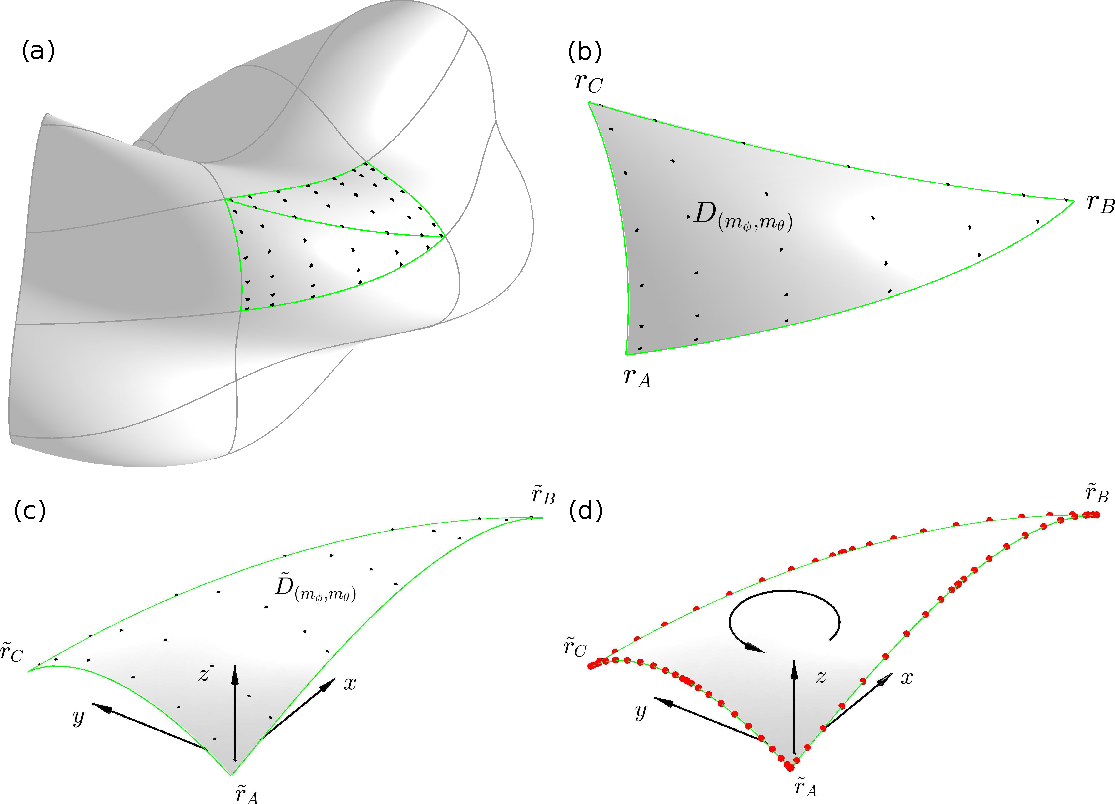
\includegraphics[height = 0.5\textwidth]{scheme.pdf}
    %\caption{}
\end{figure}

\end{frame}

\begin{noframe}\ft{More on fill $A^{\text{near}}$ and $A^{\text{self}}$: \small{kernel split quadrature}}
% observation: 

\bmp{2.6in}
\vspace{2ex}
\rb
\small{construct a harmonic polynomial approximation/extension to $\sigma(\yy)$ on $\Gamma_i$:}

\sg

\quad\com{$(\sigma(\yy), \mbf{0}) \approx -\sum_{n=1}^p\sum_{m=1}^n{(0,\nabla H^{(nm)})c^{(nm)}}$}

\sg

\com{where $H^{(nm)}(\yy) = Y_n^m(\theta,\phi)r^n$ are spherical harmonics of degree $n$. }

\sg

\rb
\small{divergence free integrand to apply surface-to-line integral conversion: }

\sg

\quad\com{$(0,\frac{\partial }{\partial \nn_\yy}\frac{1}{|\xx-\yy|})(0,\nn_\yy)(0,\nabla H^{(nm)})ds_\yy $}

\sg

\rb
\small{analytical integration along ``radial" direction: }

\sg

\quad\com{$M_n(\xx,\yy) = \int_0^1\frac{t^{n+1}}{|\xx-t\yy|^3}\mathrm{d}t$} 

\sg

\com{via recursion}

\quad\com{$M_n = \frac{ \xx \cdot \yy }{| \yy |^2}M_{n-1}+  \frac{n-1}{| \yy |^2}N_{n-2}- \left. \frac{1}{| \yy |^2}\frac{t^{n-1}}{|\xx - t \yy|} \right\rvert_0^1$}
        
\sg

\rb
\small{numerical integration along $\partial \Gamma_i$} 

\sg
\quad \who{Zhu-Veerapaneni '22}
 
\emp    
\hfill
\bmp{2.1in}
\vspace{2ex}
\pause

work in progress:

\sg

\rb
\small{Helmholtz, Stokes kernels} \who{Zhu-Jiang et al.}

\sg

\rb
\small{high aspect ratio patches, quadrilateral elements, proper single layer potential treatment} \who{Zhu-Jiang}

\sg

\rb
\small{quadrature via complete reduction} \who{Zhu-Jiang}

\hspace{4ex} \ig{height = 0.38\textwidth}{torus_GRF}


\hspace{4ex} \ig{height = 0.38\textwidth}{torus_bvp_err}

\emp 
\end{noframe}

\begin{frame}\ft{Computational tools}

\rb 
chunkie \quad \who{Askham, et al.}

\sg

\rb
fmm3dbie \quad \who{Rachh, et al.}

\sg

\rb
BIE2D, BIE3D \quad \who{Barnett}

\sg

\rb
pyBIE2D \quad \who{Stein}

\sg

\rb
SCTL, BIEST \quad \who{Malhotra}

\sg

\rb
ves3d \quad \who{Malhotra, Lu, et al.}

\sg

\rb
Bempp \quad \who{Betcke et al.}

\rb
$\cdots$

\sg

\end{frame}

\begin{frame}\ft{Resources}  % RRRRRRRRRRRRRRRRRRRRRRRRRRRRRRRRRRRRRRRRRRRRRRR

Many numerical analysis (mathematics heavy). Somewhat accessible:

\hg

\rb {\em Linear Integral Equations}, R. Kress, (1999, Springer). Ch. 6 \& 12.

\hg

\rb {\em The Numerical Solution of Integral Equations of the Second Kind},
K. E. Atkinson, (1997, CUP).

% *** add Sauter-Schwab

% *** Ladyzhenskaya, Hsiao--Wendland for Stokes?


\vg

Fewer on the practical/tutorial side, few with last 15 years of progress:

\hg

\rb ``High-order accurate methods for Nystr\"om discretization of integral equations on smooth curves in the plane'', S Hao, AH Barnett, PG Martinsson, P Young.
{\em Adv. Comput. Math.} {\bf 40}, 245--272 (2014).

\hfill \com{various quadratures for logarithmic singularities,
  for, eg, SLP, Helmholtz}

\hg

\rb ``Solving integral equations on piecewise smooth boundaries using the RCIP method: a tutorial'', J Helsing. (2013).

\hg

\rb \url{https://users.flatironinstitute.org/~ahb/BIE/}

\hg

\rb \url{https://github.com/ahbarnett/BIEbook} \hfill \com{in progress\dots}

\end{frame}


\end{document}
